\subsection{L2L2}

The L2L2 dataset consists of vertices produced when tracks do not pass through Layer 1 and their projections back to Layer 1 are within 1.5~mm of the beam (outside the active silicon region). This dataset will most likely require the most work to remove the background events, and preliminary studies with the small number of statistics have been unsuccessful. 

\subsubsection{Cuts}

The general cuts applied to the L2L2 dataset, after first requiring that track projections do not extend to the active region of Layer 1, are listed in Table~\ref{l2l2_cuts}.

\begin{table}[H]
\caption{Cuts applied to the L2L2 datasets.}
\label{l2l2_cuts}
\centering
\begin{tabular}{lllllll}
\toprule
%\multicolumn{2}{c}{Name} \\
%\cmidrule(r){1-2}
Cut type & Cut & Cut Value &  $\%$killed &  $\%$killed core & $\%$killed tails\\
\midrule
track & Fit quality & track $\chi^{2}<30$ & 44 & 66 & 44 \\
track & Max track momentum &  $P_{trk}<75\%E_{beam}$ & 15 & 14 & 15 \\
track & Isolation &   & 22 & 34 & 22 \\
vertex & beamspot constraint & bsc$\chi^{2}<10$  & 47 & 36 & 47 \\
vertex & beamspot - unconstrained & bsc$\chi^{2}$-unc$\chi^2<5$  & 18 & 0 & 19 \\
vertex & maximum $P_{sum}$ &  $<115\%E_{beam}$ & 1 & 6 & 1 \\
ecal & Ecal SVT matching & $\chi^2<10$  & 30 & 73 & 29 \\
ecal & track Ecal timing & $<4$ns  & 7 & 0 & 8 \\
ecal & 2 cluster time diff & $<2$ns  & 8 & 0 & 8 \\
physics & momentum asymmetry & $<0.4$  & 4 & 0 & 4 \\
physics & e+ track d0 & $<1.5$mm  & 21 & 33 & 21 \\
event & max shared hits amongst tracks & $<4$ shared hits  & 21 & 50 & 21 \\
\bottomrule
\end{tabular}
\end{table}

The geometric acceptance of the cuts in the L2L2 dataset leave a core fraction of background events well beyond the target at approximately 30~mm downstream. The only modifications to previously applied cuts are that both tracks use a modified isolation cut by looking at the isolation at Layer 2 and the tracks do not share 4 hits with any other track in the event.  The kink cuts appeared to not remove events from this dataset, but other options will need to be explored after unblinding. 

\subsubsection{Vertex reconstruction efficiency, $\epsilon_{vtx}$}

The L2L2 dataset is most efficient for long-lived heavy photons with detached vertices farther downstream than any of the other datasets. The efficiency in terms of mass and z vertex position is fit using the Crystal Ball function as described in Equation~\eqref{eq:cbfunction}. The parameters of fit as a function of mass are shown in Equation~\eqref{eq:parsEpsVtxL2L2}.

\begin{eqnarray*}
\label{eq:parsEpsVtxL2L2}
N & = & -0.3623+30.88m-374.7m^2\\
z_{mean} & = & -71.7603+7733.51m-131569m^2+827080m^3\\
\sigma & = & -4.058-813m-8947m^2\\
\end{eqnarray*}

If the backgrounds can be removed from the L2L2 dataset, then the zCut for this dataset can essentially cover the entire range of z values to the first layer. If some background events at lower z values cannot be removed, then it may still be possible to recover most of the efficiency of this dataset by optimizing the zCut based on the L2L2 vertex reconstruction efficiency. The efficiency for these events turns on downstream. One can propose potential zCuts where the turn on of the efficiency passes various efficiency thresholds. The corresponding possible zCut values as the efficiency surpasses 2~$\%$,5~$\%$, and 10~$\%$ are shown in Figure~\ref{fig:proposedZ_L2L2}.

\begin{figure}[H]
  \centering
     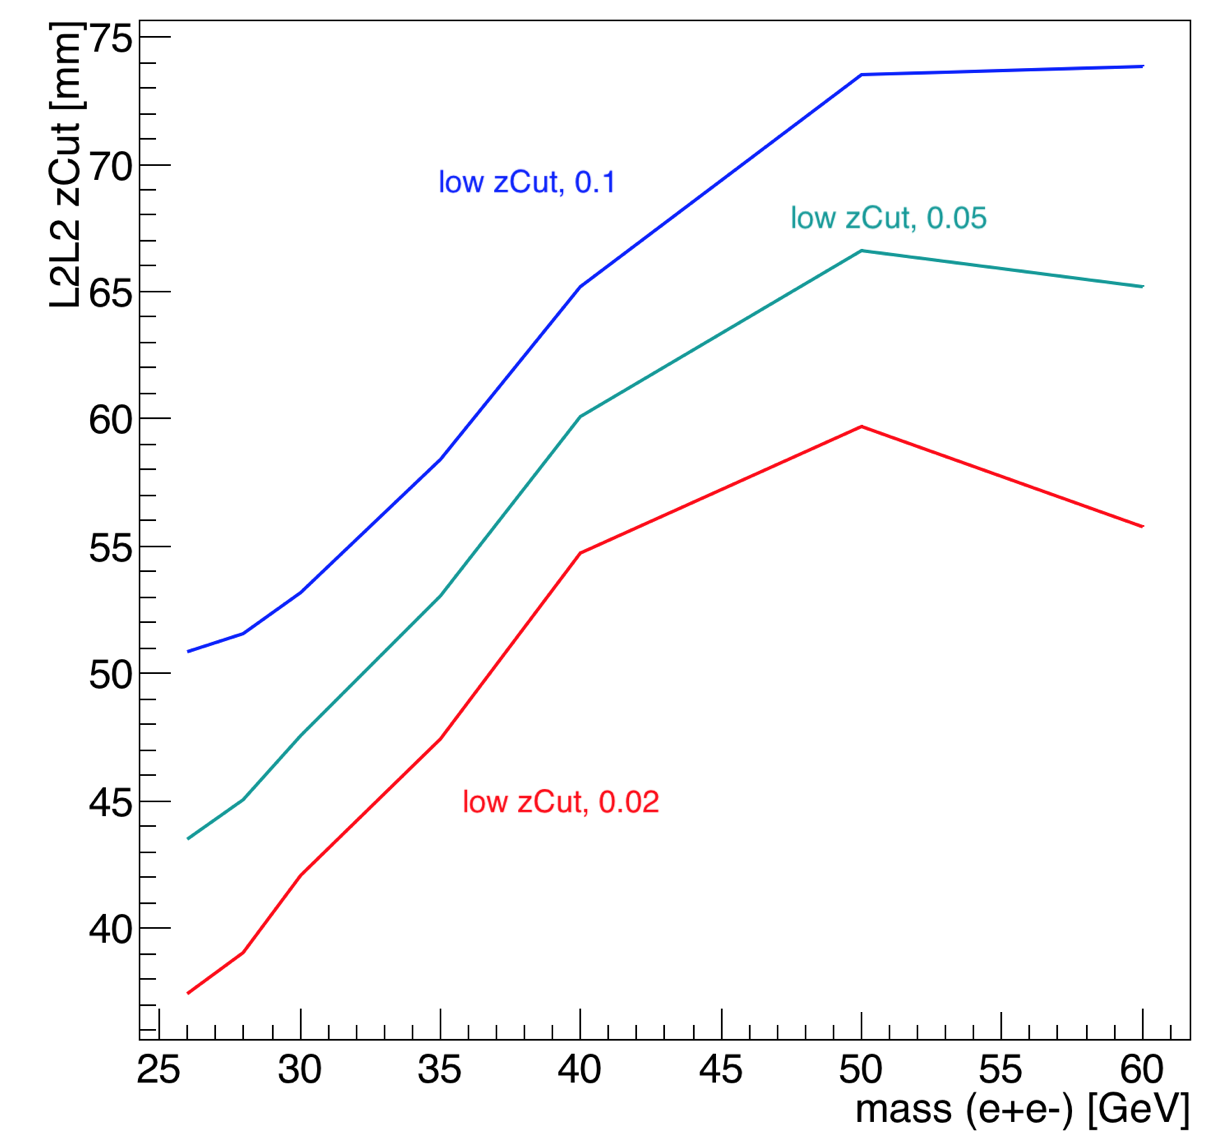
\includegraphics[width=0.8\textwidth]{plots/L2L2_proposedZcut.png}
  \caption{This is the proposed zCut for the L2L2 dataset based on the efficiency curves. The three lines represent the turn on efficiency for the L2L2 dataset for the efficiency values corresponding to 2$\%$, 5$\%$, and 10$\%$.}
  \label{fig:proposedZ_L2L2}
\end{figure} 

In order to fully realize the contribution of the L2L2 dataset to the overall reach, the high z background must be removed. 

\subsubsection{Mass resolution}

As we fit the residual heavy photon reconstructed masses for the L1L1 and L1L2 datasets, we apply the same methodology to the L2L2 dataset. Reconstructed masses are shown in the Figure~\ref{fig:l2l2_mfit}.

\begin{figure}[H]
  \centering
     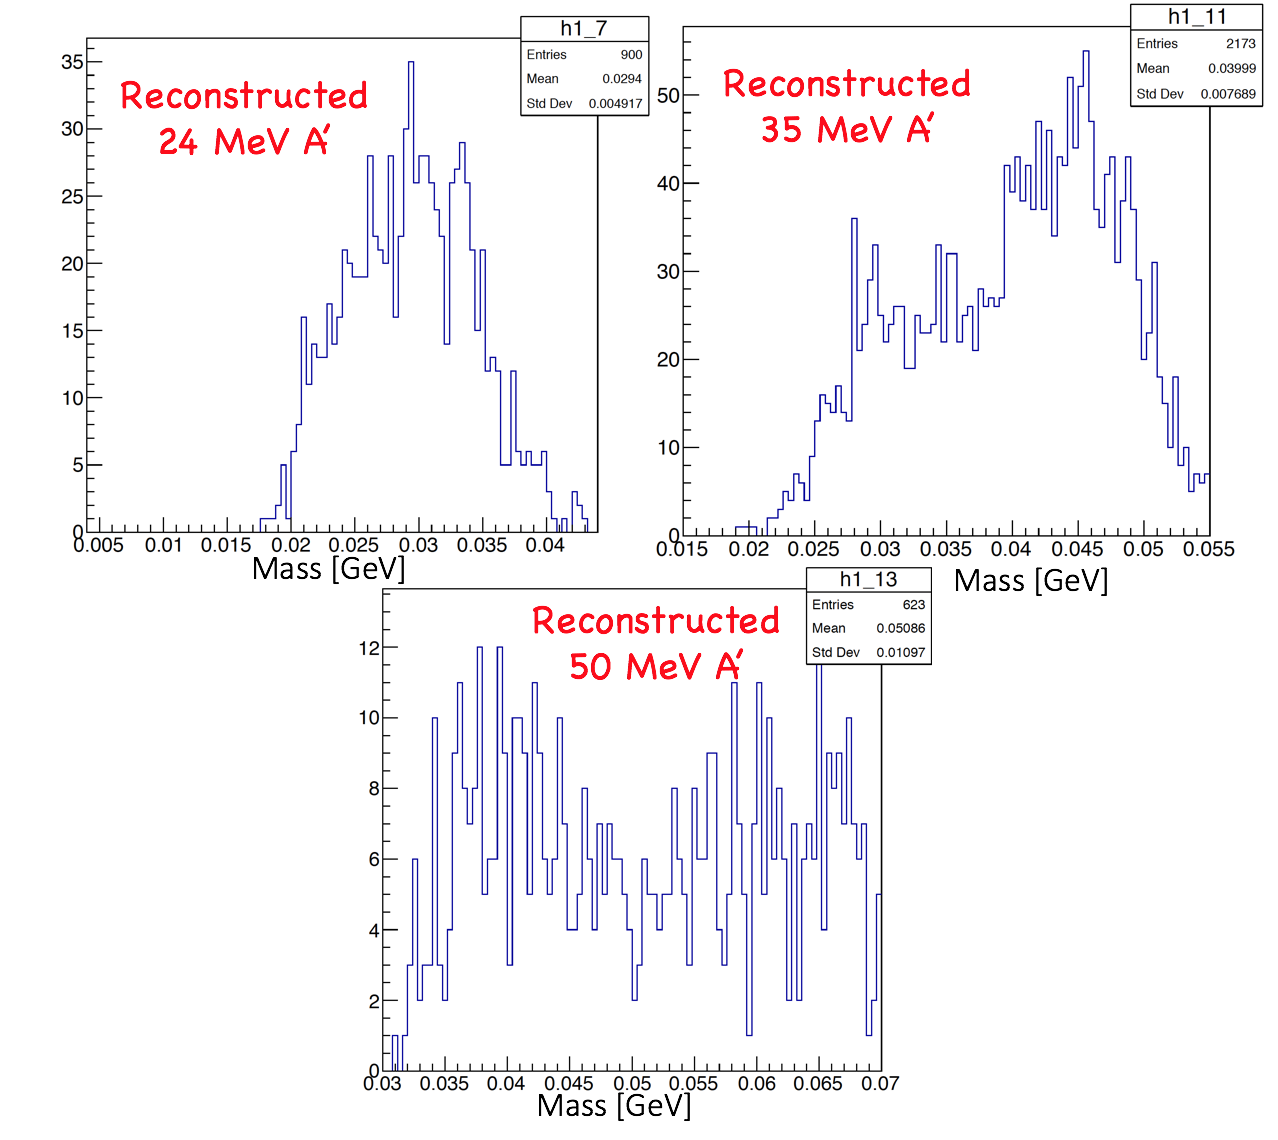
\includegraphics[width=0.8\textwidth]{plots/L2L2MassFit.png}
  \caption{The reconstructed heavy photon masses from Monte Carlo for the L2L2 dataset. Not only do the masses appear to reconstruct the wrong place, but the width of distributions indicates that we may not have the resolution to see a signal at all.}
  \label{fig:l2l2_mfit}
\end{figure} 

As shown in Figure~\ref{fig:l2l2_mfit}, in order to use the L2L2 dataset, we must improve our mass resolution. Not only are we unable to reconstruct the masses in the correct location, but we appear to lack the resolution to resolve a mass without Layer 1 at all. If we can understand and address this problem then it may be possible to recover some use of the L2L2 dataset, but without this improvement, we will not be able to reliably reconstruct any heavy photons in the event sample. For further reach calculations, the mass resolution will take the optimistic scenario and utilize the L1L2 mass resolution (in the scenario that we can solve the problem with the L2L2 mass resolution). 

\subsubsection{Accidentals}

When looking at accidentals, the same strategy was applied as previously mentioned to choose out of time events. In total, 10 events across the six beam buckets remain. This could indicate that in the dataset as selected, we may expect $3.3\pm1$ event. This rate is higher than other accidental rates, but this may also change when the L2L2 selection criteria for general vertex events is improved.

\subsubsection{Projected reach}

The reconstructed z vertex versus the mass for the L2L2 dataset is shown in its current state in Figure~\ref{fig:zVm_L2L2_0p5}.

\begin{figure}[H]
  \centering
     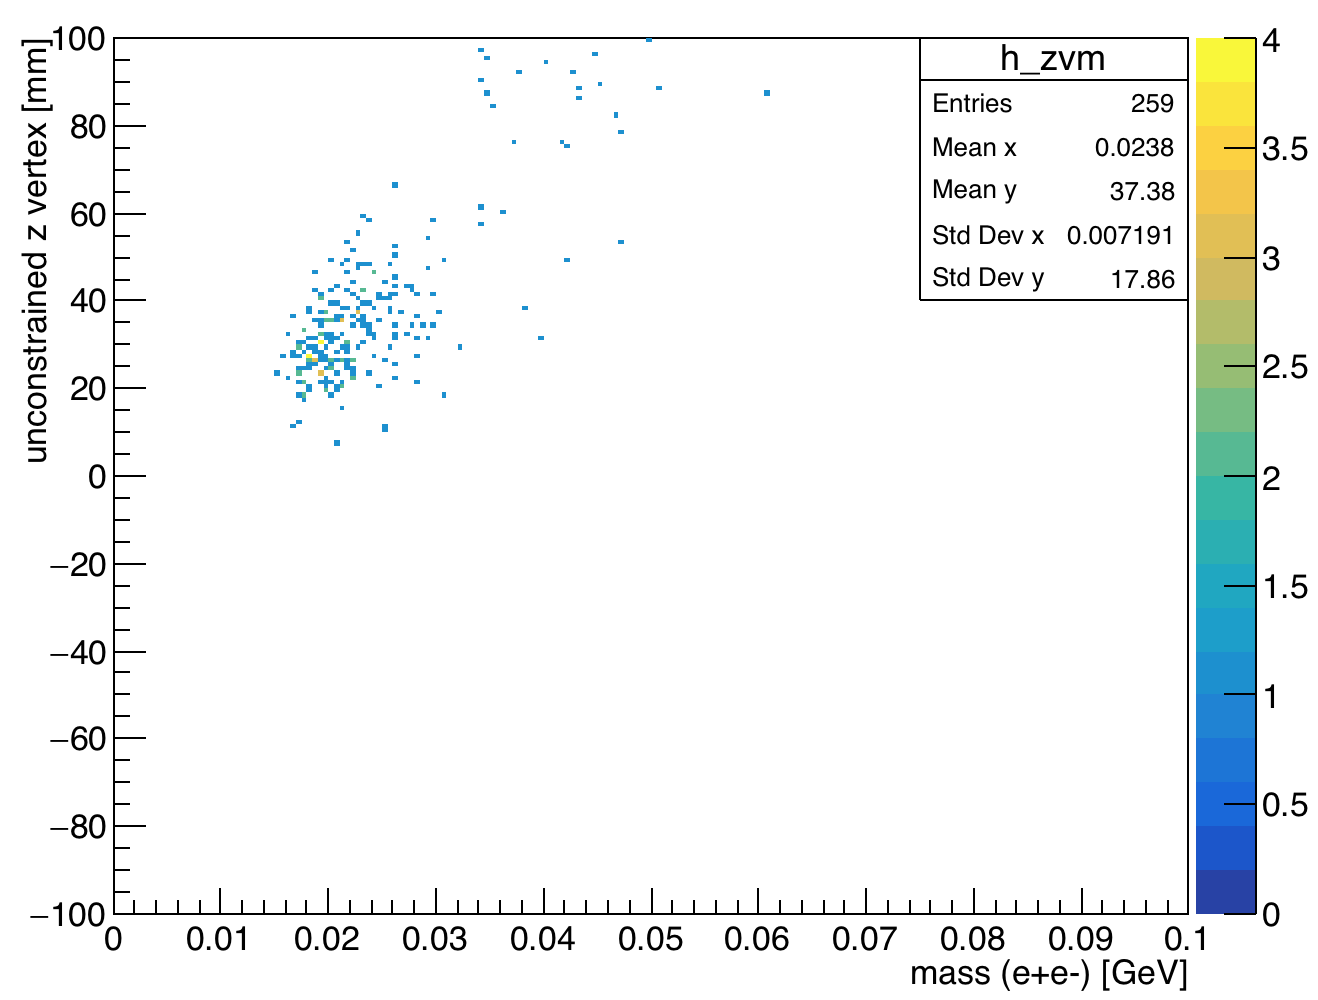
\includegraphics[width=0.8\textwidth]{plots/zVm_L2L2.png}
  \caption{Reconstructed z vertex as a function of mass for the L2L2 dataset with the first layer of the SVT at 0.5~mm from the beam.}
  \label{fig:zVm_L2L2_0p5}
\end{figure} 

The events reconstructed in the current L2L2 dataset are a background that must be fully characterized when unblinding. Assuming that we can remove the high z background and integrating from the target position to Layer 1, we could anticipate the upper limit improvement by adding the L2L2 dataset. 

\begin{figure}[H]
  \centering
     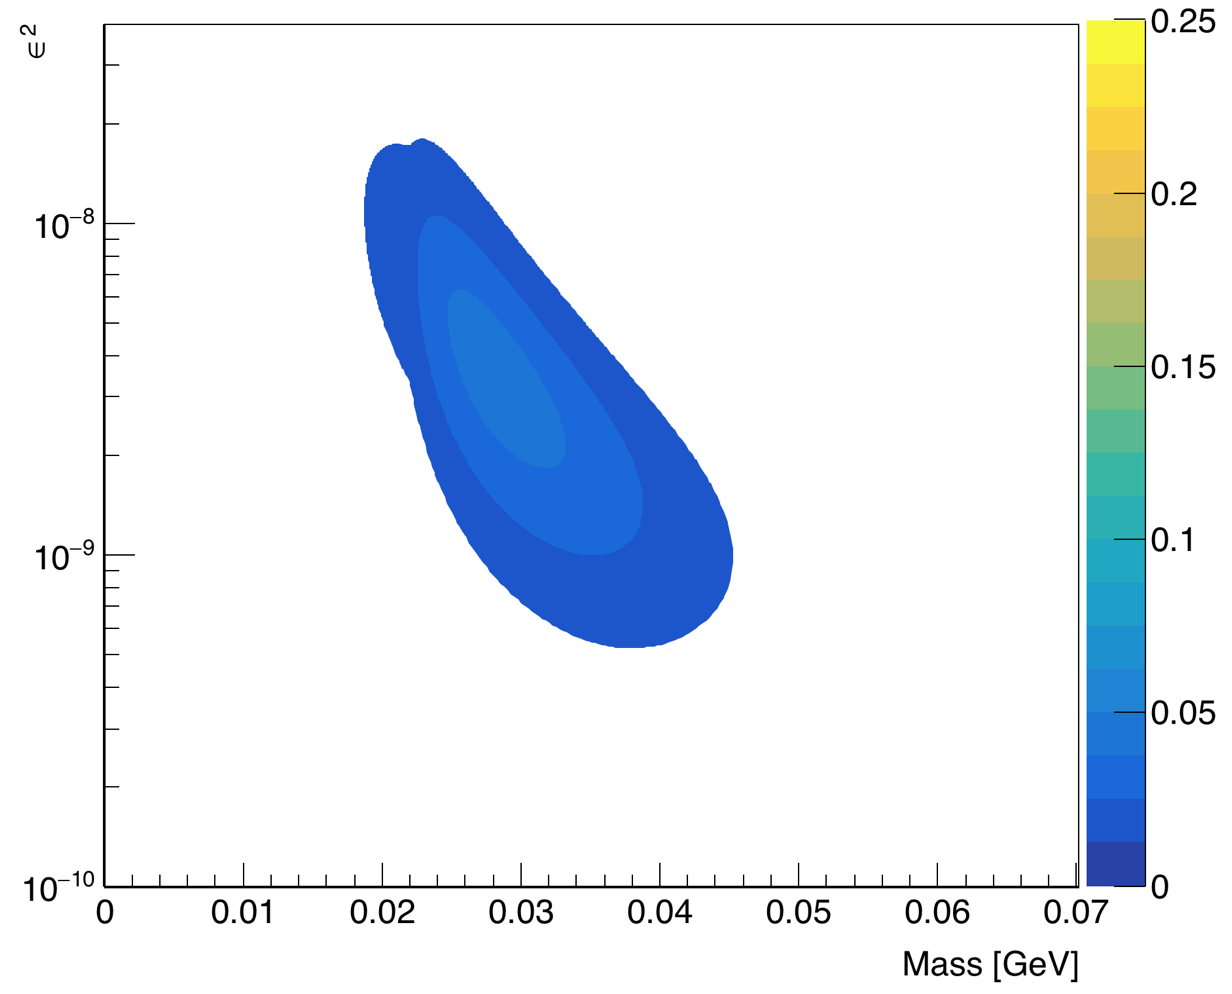
\includegraphics[width=0.8\textwidth]{plots/reachL2L2.png}
  \caption{The expected signal yield for the L2L2 0.5~mm 100$\%$ dataset. This is an upper limit estimate that assumes we can remove the background in the L2L2 dataset. }
  \label{fig:reachL2L2}
\end{figure} 


The L2L2 dataset improves the reach somewhat in the region of 20-40~MeV masses. While the efficiency of the L2L2 dataset improves at larger z vertices, the heavy photon production begins to supress in this region. 

